\documentclass[12pt]{article}
\usepackage{blindtext}
\usepackage[en,bordered]{uni-style}
\usepackage{uni-math}
\usepackage{physics}
\usepackage{amssymb}
\usepackage{capt-of}
\usepackage{karnaugh-map}
\usepackage{neuralnetwork}
\usepackage{tikz}
\tikzstyle{mynode}=[thick,draw=blue,fill=blue!20,circle,minimum size=22]


\usetikzlibrary{calc}

\def\layersep{3cm}
\newcommand\nn[1]{
    % Input layer
    \foreach \y in {1,...,2}
        \node[neuron, fill=green!40] (i\y-#1) at (0,\y+1) {$i\y$};

    % Hidden layer
    \foreach \y in {1,...,4}
        \path node[neuron, fill=blue!40] (h\y-#1) at (\layersep,\y) {$h\y$};

    % Output node
    \node[neuron, fill=red!40] (o-#1) at (2*\layersep,2.5) {$o$};

    % Connect every node in the input layer with every node in the hidden layer.
    \foreach \source in {1,...,2}
        \foreach \dest in {1,...,4}
            \path (i\source-#1) edge (h\dest-#1);

    % Connect every node in the hidden layer with the output layer
    \foreach \source in {1,...,4}
        \path (h\source-#1) edge (o-#1);
}

\makeatletter
\newcommand*{\rom}[1]{\expandafter\@slowromancap\romannumeral #1@}
\makeatother

\DeclareMathOperator*{\argmax}{arg\,max}
\DeclareMathOperator*{\argmin}{arg\,min}
\title{Intruduction to Machine Learning}
\prof{Dr \,S.Amini}
\subject{Homework 3}
\info{
    \begin{tabular}{lr}
        Amirreza Velae & 400102222\\
        github    & \href{https://github.com/amirrezavelae}{repository}\\
    \end{tabular}
    }
    \date{\today}
    % \usepackage{xepersian}
    % \settextfont{Yas}
    \usepackage{uni-code}
    
\begin{document}
\maketitlepage
\maketitlestart

\section{Design simple neural network}
Design a simple neural network with one hidden-layer that implements the following function:
\begin{gather*}
    (A\vee \bar{B}) \oplus (\bar{C} \vee \bar{D})
\end{gather*}
Draw the network and determine all its weights.
\begin{qsolve}
\begin{gather*}
    (A\vee \bar{B}) \oplus (\bar{C} \vee \bar{D}) = ((A\vee \bar{B}) \wedge (C \wedge D)) \vee ((\bar{A} \wedge B) \wedge (\bar{C} \vee \bar{D}))\\
\end{gather*}
If you plot the karnaugh map  for this special function, it looks like this:
\begin{gather*}
\begin{karnaugh-map}[4][4][1][$AB$][$CD$]
\minterms{1,5,9,12,14,15}
\maxterms{0,2,3,4,6,7,8,10,11,13}
\implicant{1}{5}
\implicant{15}{14}
\implicant{12}{12}
\implicant{9}{9}
\end{karnaugh-map}
\end{gather*}
so the function can be simplified to:
\begin{gather*}
    (\bar{A} \wedge B) \vee (C \wedge D) - (\bar{A} \wedge B \wedge C \wedge D)\\
    = (\bar{A} \wedge B \wedge \bar{C}) \vee (\bar{A} \wedge B \wedge C \wedge \bar{D}) \vee (A \wedge C \wedge D) \vee (\bar{A} \wedge \bar{B} \wedge C \wedge D)
\end{gather*}
we can say:
\begin{gather*}
    h_1 = \bar{A} \wedge B \wedge \bar{C} =  w_{1}^{T} x + b_1 ,\; \begin{cases}
        w_1 = \begin{bmatrix}
            -1 & 1 & 1 & 0 \\
        \end{bmatrix} \\
        b_1 = -1.5
    \end{cases}
\end{gather*}
\splitqsolve
\begin{gather*}
    A \wedge C \wedge D =  w_{2}^{T} x + b_2 , \; \begin{cases}
        w_2 = \begin{bmatrix}
            1 & 0 & 1 & 1 \\
        \end{bmatrix} \\
        b_2 = -2.5
    \end{cases} \\
    \bar{A} \wedge B \wedge C \wedge \bar{D} =  w_{3}^{T} x + b_3 , \; \begin{cases}
        w_3 = \begin{bmatrix}
            -1 & 1 & 1 & -1 \\
        \end{bmatrix} \\
        b_3 = -1.5
    \end{cases} \\
    \bar{A} \wedge \bar{B} \wedge C \wedge D =  w_{4}^{T} x + b_4 , \; \begin{cases}
        w_4 = \begin{bmatrix}
            -1 & -1 & 1 & 1 \\
        \end{bmatrix} \\
        b_4 = -1.5
    \end{cases} \\
    y = h_1 \vee h_2 \vee h_3 \vee h_4 =  w_{5}^{T} x + b_5 , \; \begin{cases}
        w_5 = \begin{bmatrix}
            1 & 1 & 1 & 1 \\
        \end{bmatrix} \\
        b_5 = -3.5
    \end{cases}
\end{gather*}
So the MLP model for $(A\vee \bar{B}) \oplus (\bar{C} \vee \bar{D})$ looks look like this:
\begin{align*}
    \begin{neuralnetwork}[height=5]
        \newcommand{\x}[2]{$x_#2$}
        \newcommand{\y}[2]{$\hat{y}_#2$}
        \newcommand{\hfirst}[2]{\small $h_#2$}
        \inputlayer[count=4, bias=true, title=Input\\layer, text=\x]
        \hiddenlayer[count=4, bias=true, title=Hidden layer, text=\hfirst] \linklayers
        \outputlayer[count=1, title=Output\\layer, text=\y] \linklayers
    \end{neuralnetwork}
\end{align*}
Where every link is weighted via $w_i$ or $b_i$. Also a good activation function is heaviside function.
\end{qsolve}

\section{Vector Derivative}
Consider following function:
\begin{gather*}
    \mathbf{f_1}(\begin{bmatrix}
        x_1 \\
        x_2
    \end{bmatrix}) =
    \begin{bmatrix}
        \frac{1}{\pi} sin(\pi x_2) \\
        e^{x_1 -1}x^{2}_2          \\
        x_1 x_2
    \end{bmatrix}
    , \; \; \;
    \mathbf{f_2}(\begin{bmatrix}
        x_1 \\
        x_2 \\
        x_3
    \end{bmatrix}) =
    \begin{bmatrix}
        x_1 + x_2 + x_3             \\
        {x_1}^2 + {x_2}^2 + {x_3}^2 \\
    \end{bmatrix}
\end{gather*}
\begin{align*}
    \mathbf{f(x)} = (\mathbf{f_2 \circ  f_1})(\mathbf{x})
\end{align*}
Determine $\pdv{\mathbf{f}}{\mathbf{x}}$ at point $\mathbf{x} = \begin{bmatrix}
        1 \\
        2
    \end{bmatrix}$ \\
*Note that your solution must follow the methods mentioned in the course slides.
\begin{qsolve}
    In this specific example, n=m. Thus it is possible to calculate the Jacobian matrix of the function f(x) as follows:
    \begin{gather*}
        \begin{bmatrix}
            \pdv{f_1}{x_1} & \pdv{f_1}{x_2} \\
            \pdv{f_2}{x_1} & \pdv{f_2}{x_2} \\
        \end{bmatrix}
        \begin{bmatrix}
            x_1 \\
            x_2 \\
        \end{bmatrix}
    \end{gather*}
    First thing to do is to, we have to get $v_1$ and $v_2$ at point $\mathbf{x} = \begin{bmatrix}
            1 \\
            2
        \end{bmatrix}$:
    \begin{gather*}
        v_1 = e_1 = \begin{bmatrix}
            1 \\
            0 \\
        \end{bmatrix}
        \; \; \; \; \;
        v_2 = e_2 = \begin{bmatrix}
            0 \\
            1 \\
        \end{bmatrix}
    \end{gather*}
    For $\mathbf{f_1}$:
    \begin{gather*}
        J_{\mathbf{f_1}}(\mathbf{x}) =
        \begin{bmatrix}
            0                 & cos(\pi x_2)   \\
            e^{x_1 -1}x^{2}_2 & 2e^{x_1 -1}x_2 \\
            x_2               & x_1            \\
        \end{bmatrix}
    \end{gather*}
    and for $\mathbf{f_2}$:
    \begin{gather*}
        J_{\mathbf{f_2}}(\mathbf{x}) =
        \begin{bmatrix}
            1    & 1    & 1    \\
            2x_1 & 2x_2 & 2x_3 \\
        \end{bmatrix}
    \end{gather*}
    at point $\mathbf{x} = \begin{bmatrix}
            1 \\
            2
        \end{bmatrix}$:
    \begin{gather*}
        x_2 = \mathbf{f_1(x_1)} = \begin{bmatrix}
            \frac{1}{\pi} sin(2 \pi) \\
            e^{1 -1}2^{2}            \\
            2                        \\
        \end{bmatrix} = \begin{bmatrix}
            0 \\
            4 \\
            2 \\
        \end{bmatrix}
        \; \; \; \; \;
        J_{\mathbf{f_1}}(\mathbf{x}) =
        \begin{bmatrix}
            0             & cos(2 \pi) \\
            e^{1 -1}2^{2} & 2e^{1 -1}2 \\
            2             & 1          \\
        \end{bmatrix}
        =
        \begin{bmatrix}
            0 & 1 \\
            4 & 4 \\
            2 & 1 \\
        \end{bmatrix}
    \end{gather*}
    then for new $v_1$ and $v_2$:
    \begin{gather*}
        v_1 = J_{\mathbf{f_1}}(\mathbf{x}) v_1 =
        \begin{bmatrix}
            0 & 1 \\
            4 & 4 \\
            2 & 1 \\
        \end{bmatrix}
        \begin{bmatrix}
            1 \\
            0 \\
        \end{bmatrix}
        =
        \begin{bmatrix}
            0 \\
            4 \\
            2 \\
        \end{bmatrix}
        \; \; \; \; \;
        v_2 = J_{\mathbf{f_1}}(\mathbf{x}) v_2 =
        \begin{bmatrix}
            0 & 1 \\
            4 & 4 \\
            2 & 1 \\
        \end{bmatrix}
        \begin{bmatrix}
            0 \\
            1 \\
        \end{bmatrix}
        =
        \begin{bmatrix}
            1 \\
            4 \\
            1 \\
        \end{bmatrix}
    \end{gather*}
    For $\mathbf{f_2}$:
    \begin{gather*}
        x_2 = \mathbf{f_2(x_1)} = \begin{bmatrix}
            0 + 4 + 2  \\
            0 + 16 + 4 \\
        \end{bmatrix} = \begin{bmatrix}
            6  \\
            20 \\
        \end{bmatrix}
        \; \; \; \; \;
        J_{\mathbf{f_2}}(\mathbf{x}) =
        \begin{bmatrix}
            1 & 1 & 1 \\
            0 & 8 & 4 \\
        \end{bmatrix}
    \end{gather*}
    then for new $v_1$ and $v_2$:
    \begin{gather*}
        v_1 = J_{\mathbf{f_2}}(x_2) v_1 =
        \begin{bmatrix}
            1 & 1 & 1 \\
            0 & 8 & 4 \\
        \end{bmatrix}
        \begin{bmatrix}
            0 \\
            4 \\
            2 \\
        \end{bmatrix}
        =
        \begin{bmatrix}
            6  \\
            40 \\
        \end{bmatrix}
        \; \; \; \; \;
        v_2 = J_{\mathbf{f_2}}(x_2) v_2 =
        \begin{bmatrix}
            1 & 1 & 1 \\
            0 & 8 & 4 \\
        \end{bmatrix}
        \begin{bmatrix}
            1 \\
            4 \\
            1 \\
        \end{bmatrix}
        =
        \begin{bmatrix}
            6  \\
            36 \\
        \end{bmatrix}
    \end{gather*}
    \splitqsolve
    Thus:
    \begin{gather*}
        J_f(\mathbf{x}) = \begin{bmatrix}
            v_{1} & v_{2} \\
        \end{bmatrix}
        = \begin{bmatrix}
            6  & 6  \\
            40 & 36 \\
        \end{bmatrix}
    \end{gather*}
\end{qsolve}

\section{One Convolutional Layer}
Consider we have one convolutional layer with following equation:
\begin{gather*}
    \begin{bmatrix}
        z_{1}  \\
        \vdots \\
        z_{m}  \\
    \end{bmatrix}
    = \begin{bmatrix}
        k_1 & \cdots & k_d    &        &        &     \\
            & k_1    & \cdots & k_d    &        &     \\
            &        &        & \ddots &        &     \\
            &        &        & k_1    & \cdots & k_d \\
    \end{bmatrix}
    \begin{bmatrix}
        x_{1}  \\
        \vdots \\
        x_{n}  \\
    \end{bmatrix}
    + \begin{bmatrix}
        b      \\
        \vdots \\
        b      \\
    \end{bmatrix}
\end{gather*}
and also we know:
\begin{gather*}
    \pdv{L}{z_i} = \alpha_i
\end{gather*}
calculate $\pdv{L}{k_j}$ and $\pdv{L}{b}$ in terms of $x_i$ and $z_i$.
\begin{qsolve}
    \begin{gather*}
        \pdv{L}{k_j} = \sum_{i=1}^{m} \pdv{L}{z_i} \pdv{z_i}{k_j} = \sum_{i=1}^{m} \alpha_i x_{i+j-1} \\
        \pdv{L}{b} = \sum_{i=1}^{m} \pdv{L}{z_i} \pdv{z_i}{b} = \sum_{i=1}^{m} \alpha_i
    \end{gather*}
\end{qsolve}
\section{Backpropagation Algorithm}
The following image shows a two-layer neural network with two nodes in the hidden layer and one node in the output. $x_1$ and $x_2$ are two inputs to the network. Each node has a bias with value of 1.
\\
Assume that the value of the learning rate is 0.1 and the activation function is sigmoid in both hidden-layer and output-layer.
\begin{itemize}
    \item Calculate the value at nodes $\hat{y} , h_1 , h_2$ for input \{$x_1 = 0 , x_2 = 1$\}.
    \item Execute one step of backpropagation algorithm for the previous input in part (a) and output $y = 1$.
    \item Calculate the updated weights for the hidden-layer and output-layer (a total of 9 weights) by executing one step of the gradient descent algorithm.
\end{itemize}
\begin{figure}[h]
    \centering
    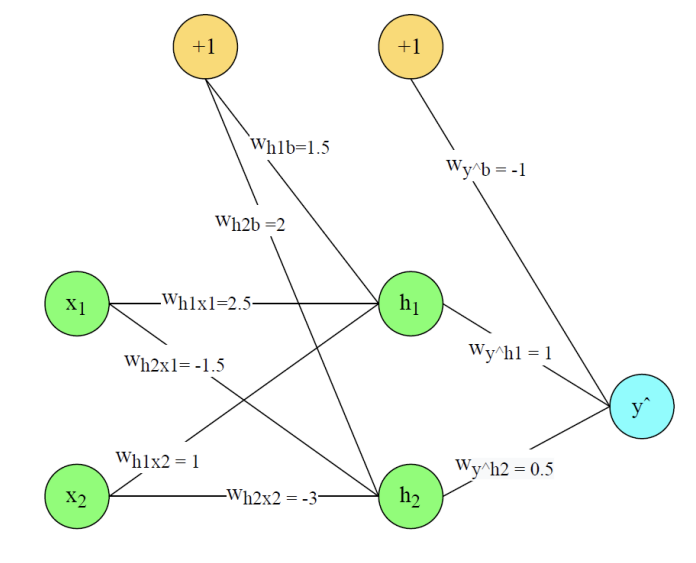
\includegraphics[width=0.5\textwidth]{Q4.png}
\end{figure}
\begin{qsolve}[Part \rom{1}]
    \begin{gather*}
        \hat{y} = \sigma(\mathbf{w_{y^{h_0}}}\mathbf{h_0} + \mathbf{w_{y^{h_1}}}\mathbf{h_1} + \mathbf{w_{y^{h_2}}}\mathbf{h_2}) \\
        h_1 = \sigma(\mathbf{w_{h_1^{x_1}}}\mathbf{x_1} + \mathbf{w_{h_1^{x_2}}}\mathbf{x_2} + \mathbf{w_{h_1^{b}}}\mathbf{b}) \\
        h_2 = \sigma(\mathbf{w_{h_2^{x_1}}}\mathbf{x_1} + \mathbf{w_{h_2^{x_2}}}\mathbf{x_2} + \mathbf{w_{h_2^{b}}}\mathbf{b}) \\
    \end{gather*}
    Given values for weights:
    \begin{gather*}
        \mathbf{w_{y^{h_0}}} = -1 \; \; \; \; \; \; \; \; \; \; \; \; \; \; \mathbf{w_{y^{h_1}}} = 1 \; \; \; \; \; \; \; \; \; \; \; \; \; \; \mathbf{w_{y^{h_2}}} = 0.5 \\
        \mathbf{w_{h_1^{x_1}}} = 2.5 \; \; \; \; \; \; \; \; \; \; \; \; \; \; \mathbf{w_{h_1^{x_2}}} = 1 \; \; \; \; \; \; \; \; \; \; \; \; \; \; \mathbf{w_{h_1^{b}}} = 1.5 \\
        \mathbf{w_{h_2^{x_1}}} = -1.5 \; \; \; \; \; \; \; \; \; \; \; \; \; \; \mathbf{w_{h_2^{x_2}}} = -3 \; \; \; \; \; \; \; \; \; \; \; \; \; \; \mathbf{w_{h_2^{b}}} = 2 \\
    \end{gather*}
    also $\mathbf{h_0} = +1$ and $\mathbf{b} = +1$.\\
    So:
    \begin{gather*}
        h_1 = \sigma(2.5 \times 0 + 1 \times 1 + 1.5 \times 1) = \sigma(1 + 1.5) = \sigma(2.5) = 0.924 \\
        h_2 = \sigma(-1.5 \times 0 + -3 \times 1 + 2 \times 1) = \sigma(-3 + 2) = \sigma(-1) = 0.268 \\
        \hat{y} = \sigma(-1 \times 1 + 1 \times 0.993 + 0.5 \times 0.268) = \sigma(-1 + 0.924 + 0.134) = \sigma(0.058) = 0.514
    \end{gather*}
\end{qsolve}
\begin{qsolve}[Part \rom{2}]
    To execute back propagation algorithm for one step, we need to calculate $\pdv{L}{\mathbf{w_{y^{h_0}}}}$, $\pdv{L}{\mathbf{w_{y^{h_1}}}}$, $\pdv{L}{\mathbf{w_{y^{h_2}}}}$, $\pdv{L}{\mathbf{w_{h_1^{x_1}}}}$, $\pdv{L}{\mathbf{w_{h_1^{x_2}}}}$, $\pdv{L}{\mathbf{w_{h_1^{b}}}}$, $\pdv{L}{\mathbf{w_{h_2^{x_1}}}}$, $\pdv{L}{\mathbf{w_{h_2^{x_2}}}}$, $\pdv{L}{\mathbf{w_{h_2^{b}}}}$.
    \begin{gather*}
        w_{t+1} = w_t - \eta \pdv{L}{w_t}\\
        \pdv{L}{w_t} = \pdv{L}{\hat{y}} \pdv{\hat{y}}{w_t} = \pdv{L}{\hat{y}} \pdv{\hat{y}}{h_0} \pdv{h_0}{w_t} + \pdv{L}{\hat{y}} \pdv{\hat{y}}{h_1} \pdv{h_1}{w_t} + \pdv{L}{\hat{y}} \pdv{\hat{y}}{h_2} \pdv{h_2}{w_t} \\
        \pdv{L}{\hat{y}} = \frac{2}{2}(\hat{y} - y) = (\hat{y} - y) = (0.514 - 1) = -0.486 \\
        \pdv{\hat{y}}{h_0} = \sigma(h_0) (1 - \sigma(h_0)) = \sigma(1) (1 - \sigma(1)) = 0.731 \times 0.269 = 0.196 \\
        \pdv{\hat{y}}{h_1} = \sigma(h_1) (1 - \sigma(h_1)) = \sigma(0.924) (1 - \sigma(0.924)) = 0.715 \times 0.075 = 0.054 \\
        \pdv{\hat{y}}{h_2} = \sigma(h_2) (1 - \sigma(h_2)) = \sigma(0.268) (1 - \sigma(0.268)) = 0.567 \times 0.732 = 0.415 \\ \\ \\
        \pdv{h_0}{w_{y^{h_0}}} = 1 \; \; \; \; \; \; \; \; \; \; \; \; \; \; \pdv{h_1}{w_{y^{h_0}}} = 0 \; \; \; \; \; \; \; \; \; \; \; \; \; \; \pdv{h_2}{w_{y^{h_0}}} = 0 \\
        \pdv{h_0}{w_{y^{h_1}}} = 0 \; \; \; \; \; \; \; \; \; \; \; \; \; \; \pdv{h_1}{w_{y^{h_1}}} = 1 \; \; \; \; \; \; \; \; \; \; \; \; \; \; \pdv{h_2}{w_{y^{h_1}}} = 0 \\
        \pdv{h_0}{w_{y^{h_2}}} = 0 \; \; \; \; \; \; \; \; \; \; \; \; \; \; \pdv{h_1}{w_{y^{h_2}}} = 0 \; \; \; \; \; \; \; \; \; \; \; \; \; \; \pdv{h_2}{w_{y^{h_2}}} = 1 \\
        \pdv{h_0}{w_{h_1^{x_1}}} = 0 \; \; \; \; \; \; \; \; \; \; \; \; \; \; \pdv{h_1}{w_{h_1^{x_1}}} = \sigma(h_1) (1 - \sigma(h_1)) x_1 = 0.924 \times 0.076 \times 1 = 0.070 \\
        \pdv{h_0}{w_{h_1^{x_2}}} = 0 \; \; \; \; \; \; \; \; \; \; \; \; \; \; \pdv{h_1}{w_{h_1^{x_2}}} = \sigma(h_1) (1 - \sigma(h_1)) x_2 = 0.924 \times 0.076 \times 1 = 0.070 \\
        \pdv{h_0}{w_{h_1^{b}}} = 0 \; \; \; \; \; \; \; \; \; \; \; \; \; \; \pdv{h_1}{w_{h_1^{b}}} = \sigma(h_1) (1 - \sigma(h_1)) = 0.924 \times 0.076 = 0.070 \\
        \pdv{h_0}{w_{h_2^{x_1}}} = 0 \; \; \; \; \; \; \; \; \; \; \; \; \; \; \pdv{h_2}{w_{h_2^{x_1}}} = \sigma(h_2) (1 - \sigma(h_2)) x_1 = 0.268 \times 0.732 \times 1 = 0.196 \\
        \pdv{h_0}{w_{h_2^{x_2}}} = 0 \; \; \; \; \; \; \; \; \; \; \; \; \; \; \pdv{h_2}{w_{h_2^{x_2}}} = \sigma(h_2) (1 - \sigma(h_2)) x_2 = 0.268 \times 0.732 \times 1 = 0.196 \\
        \pdv{h_0}{w_{h_2^{b}}} = 0 \; \; \; \; \; \; \; \; \; \; \; \; \; \; \pdv{h_2}{w_{h_2^{b}}} = \sigma(h_2) (1 - \sigma(h_2)) = 0.268 \times 0.732 = 0.196 \\
    \end{gather*}
    \splitqsolve
    \begin{gather*}
        \pdv{L}{w_{y^{h_0}}} = \pdv{L}{\hat{y}} \pdv{\hat{y}}{h_0} \pdv{h_0}{w_{y^{h_0}}} = -0.486 \times 0.196 \times 1 = -0.095 \\
        \pdv{L}{w_{y^{h_1}}} = \pdv{L}{\hat{y}} \pdv{\hat{y}}{h_1} \pdv{h_1}{w_{y^{h_1}}} = -0.486 \times 0.054 \times 1 = -0.026 \\
        \pdv{L}{w_{y^{h_2}}} = \pdv{L}{\hat{y}} \pdv{\hat{y}}{h_2} \pdv{h_2}{w_{y^{h_2}}} = -0.486 \times 0.415 \times 1 = -0.202 \\
        \pdv{L}{w_{h_1^{x_1}}} = \pdv{L}{\hat{y}} \pdv{\hat{y}}{h_0} \pdv{h_0}{w_{h_1^{x_1}}} = -0.486 \times 0.196 \times 0.070 = -0.006 \\
        \pdv{L}{w_{h_1^{x_2}}} = \pdv{L}{\hat{y}} \pdv{\hat{y}}{h_0} \pdv{h_0}{w_{h_1^{x_2}}} = -0.486 \times 0.196 \times 0.070 = -0.006 \\
        \pdv{L}{w_{h_1^{b}}} = \pdv{L}{\hat{y}} \pdv{\hat{y}}{h_0} \pdv{h_0}{w_{h_1^{b}}} = -0.486 \times 0.196 \times 0.070 = -0.006 \\
        \pdv{L}{w_{h_2^{x_1}}} = \pdv{L}{\hat{y}} \pdv{\hat{y}}{h_0} \pdv{h_0}{w_{h_2^{x_1}}} = -0.486 \times 0.196 \times 0.196 = -0.019 \\
        \pdv{L}{w_{h_2^{x_2}}} = \pdv{L}{\hat{y}} \pdv{\hat{y}}{h_0} \pdv{h_0}{w_{h_2^{x_2}}} = -0.486 \times 0.196 \times 0.196 = -0.019 \\
        \pdv{L}{w_{h_2^{b}}} = \pdv{L}{\hat{y}} \pdv{\hat{y}}{h_0} \pdv{h_0}{w_{h_2^{b}}} = -0.486 \times 0.196 \times 0.196 = -0.019 \\
    \end{gather*}
\end{qsolve}
\begin{qsolve}[Part \rom{3}]
    to calculate updated weights, we use the following formula:
    \begin{gather*}
        w_{new} = w_{old} - \eta \pdv{L}{w_{old}}
    \end{gather*}
    where $\eta = 0.1$ is the learning rate and $w_{old}$ is the weight before the update. \\
    \begin{gather*}
        w_{y^{h_0}} = -1 - 0.1 \times 0.095 = -1.0095 \\
        w_{y^{h_1}} = 1 - 0.1 \times 0.026 = 0.9974 \\
        w_{y^{h_2}} = 0.5 - 0.1 \times 0.202 = 0.4798 \\
        w_{h_1^{x_1}} = 2.5 - 0.1 \times -0.006 = 2.5006 \\
        w_{h_1^{x_2}} = 1 - 0.1 \times -0.006 = 1.0006 \\
        w_{h_1^{b}} = 1.5 - 0.1 \times -0.006 = 1.5006 \\
        w_{h_2^{x_1}} = -1.5 - 0.1 \times -0.019 = -1.4981 \\
        w_{h_2^{x_2}} = -3 - 0.1 \times -0.019 = -2.9981 \\
        w_{h_2^{b}} = 2 - 0.1 \times -0.019 = 2.0019 \\
    \end{gather*}
\end{qsolve}

\section{Model Parameters}
Consider the following two-layer convolutional network.
\begin{figure}[h]
    \centering
    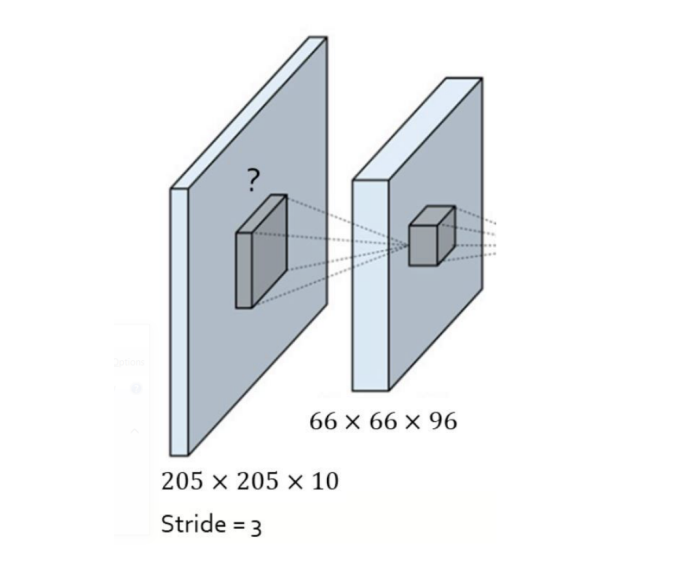
\includegraphics[width=0.5\textwidth]{Q5.png}
\end{figure}
\begin{itemize}
    \item Based on the input and output dimensions shown in the figure, determine the size of the kernel used for this operation.
    \item Determine the number of trainable parameters in this layer.
    \item Calculate the number of multiplication operations required to obtain the output.
\end{itemize}

\begin{qsolve}[Part \rom{1}]
    Via CNN we have the following formula:
    \begin{gather*}
        \frac{N - F + 2P}{S} + 1 = M
    \end{gather*}
    The input dimension is $205 \times 205 \times 10$ and the output dimension is $66 \times 66 \times 96$ and the stride is 3. \\
    The kernel size is $k \times k \times 10$ and the output dimension is $\frac{205 - k}{3} + 1 \times \frac{205 - k}{3} + 1 \times 96$ \\
    \begin{gather*}
        \frac{205 - k}{3} + 1 = 66 \\
        \frac{205 - k}{3} = 65 \\
        205 - k = 195 \\
        k = 10
    \end{gather*}
\end{qsolve}
\begin{qsolve}[Part \rom{2}]
    Total trainable parameters of this CNN is equal to $(h_w \times w_w \times C + 1)\times D$.\\
    So in this specific problem, we have $((10\times 10 \times 10)+1)\times 96 = 96096$ trainable parameters.
\end{qsolve}

\begin{qsolve}[Part \rom{3}]
    Total number of equations regarding to convolution formula:\\
    \begin{align*}
        z_{pqd} = \phi (b_c + \sum_{c=0}^{C-1}\sum_{i=0}^{h_w -1}\sum_{j=0}^{w_w -1}w_{ijkc} \; \hat{x}_{(h_s\times p+i)(w_s\times q+j)c})
    \end{align*}
    is 2 for calculating indices of $\mathbf{x}$ and one for multiplying $w$ and $x$. if we ignore the calculation of indices of $x$, then we have $(66 \times 66 \times 96)\times (10 \times 10 \times 10) = 418176000$ multiplying operations.
\end{qsolve}

\makeendpage
\end{document}